\documentclass{article}
\usepackage{amsmath,amsfonts,amssymb}
\usepackage{tikz,pgfplots}
\usepackage[paperheight=4cm,paperwidth=6cm]{geometry}
\usetikzlibrary{arrows,arrows.meta,bending,calc,decorations,shadings,shadows,shapes,shapes.arrows,shapes.geometric}
\usetikzlibrary{calc,fadings,decorations.pathreplacing,patterns}
\usepgfplotslibrary{units,fillbetween,groupplots,colorbrewer}
\usetikzlibrary{pgfplots.colorbrewer,}
\usepackage{pgfplotstable}
\pgfdeclaredecoration{penciline}{initial}{
	\state{initial}[width=+\pgfdecoratedinputsegmentremainingdistance,
	auto corner on length=1mm,]{
		\pgfpathcurveto%
		{% From
			\pgfqpoint{\pgfdecoratedinputsegmentremainingdistance}
			{\pgfdecorationsegmentamplitude}
		}
		{%  Control 1
			\pgfmathrand
			\pgfpointadd{\pgfqpoint{\pgfdecoratedinputsegmentremainingdistance}{0pt}}
			{\pgfqpoint{-\pgfdecorationsegmentaspect
					\pgfdecoratedinputsegmentremainingdistance}%
				{\pgfmathresult\pgfdecorationsegmentamplitude}
			}
		}
		{%TO 
			\pgfpointadd{\pgfpointdecoratedinputsegmentlast}{\pgfpoint{1pt}{1pt}}
		}
	}
	\state{final}{}
}

\begin{document}
	\thispagestyle{empty}
	\begin{tikzpicture}[remember picture,overlay]
		% You can see the border of the page node with this:
		\draw[thick] (current page.south west) rectangle (current page.north east);
		\draw[decorate,style=help lines] (-1,-3) grid[step=1cm] (4,1);
		%\draw (0,0) node[anchor=south] {.};
		
\begin{scope}[yshift=-1.5cm,xshift=3cm]
	\pgfmathsetmacro{\cubex}{4}
	\pgfmathsetmacro{\cubey}{0.2}
	\pgfmathsetmacro{\cubez}{3}
	\draw[fill=gray!50!green] (0,0,0) -- ++(-\cubex,0,0) -- ++(0,-\cubey,0) -- ++(\cubex,0,0) -- cycle;
	\draw[fill=gray!50!green] (0,0,0) -- ++(0,0,-\cubez) -- ++(0,-\cubey,0) -- ++(0,0,\cubez) -- cycle;
	\draw[fill=gray!50!green] (0,0,0) -- ++(-\cubex,0,0) -- ++(0,0,-\cubez) -- ++(\cubex,0,0) -- cycle;
\end{scope}
\begin{scope}[decoration=penciline, decorate]
 \draw[decorate,thick,rotate=5,opacity=0.7] (-0.3cm,-0.1cm) rectangle (1,-1);
 \draw[decorate,thick,rotate=0,opacity=0.5,rotate around={12:(-0.1cm,-0.8cm)}](-0.1cm,-0.8cm) rectangle (1,-1);
\end{scope}




	\end{tikzpicture}
\end{document}